DeepLearning技術の発展に伴い,車載や産業,スマートホームといった多くの分野への活用が期待されている.
特に,エッジデバイス上で処理するエッジAIは,2023年現在,産業分野を中心に活用が進み,車載分野における自動運転は2030年以降に活用が広まるものと予想されている.

図\ref{edge_ai_market}はエッジAI関連市場の予測を示すものである.
2035年頃まではスマートカメラやスマートホームなど産業・民生分野を中心に成長し,2030年ごろから自動運転が実用化されることが予測されている.

なお本グラフは,Appendix \ref{appendix_market}に示す数値をもとに,年平均成長率(CAGR)で各年の数値を補完したものである.

\begin{figure} [H]
	\begin{center}
		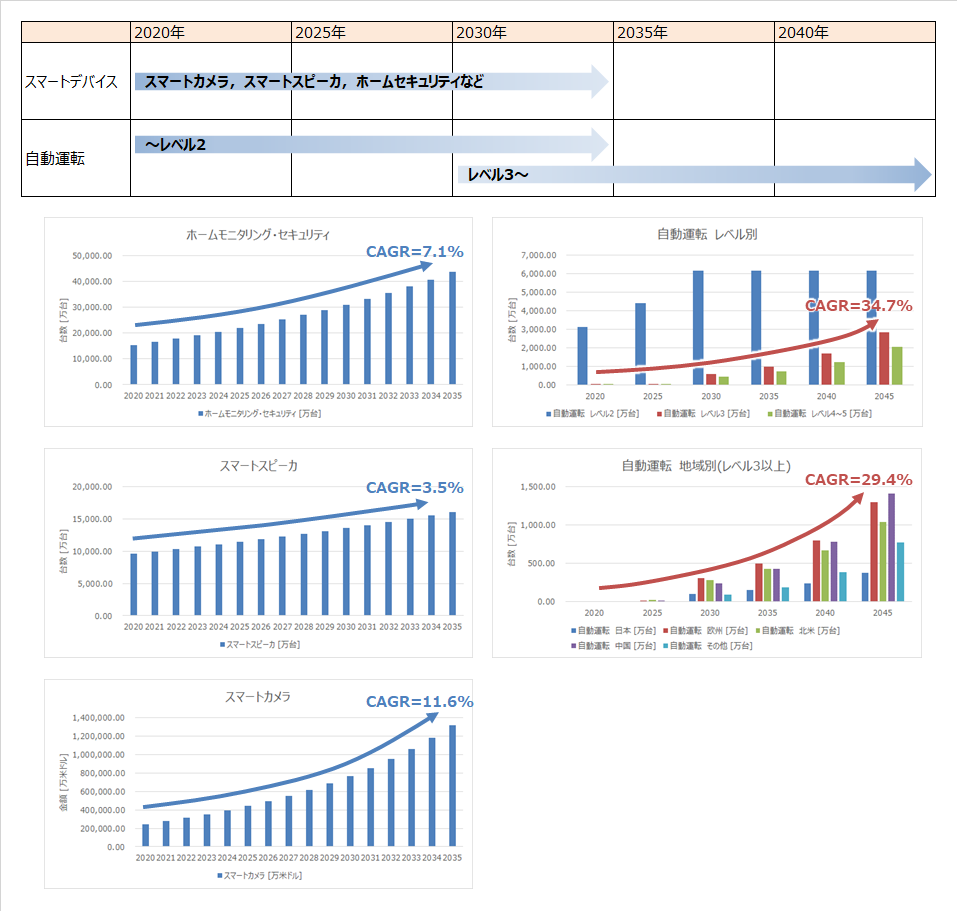
\includegraphics[clip, height=15cm, bb=-100 0 957 911]{data/figure/edge_ai_market.png}
		\caption{エッジAI関連市場の動向}
		\label{edge_ai_market}
	\end{center}
\end{figure}

AI処理をエッジ化することにより,下記のような効果が期待できる.

\begin{itemize}
	\item リアルタイム性・低遅延
	\begin{itemize}
		\item ネットワーク通信を介さないデータ処理で即時に応答
	\end{itemize}
	\item 情報漏洩リスクの低減
	\begin{itemize}
		\item クラウド利用がない為,機密情報の漏洩リスクを低減
	\end{itemize}
	\item 通信負荷と通信コストの低減
	\begin{itemize}
		\item データ処理がエッジで完結することにより,ネットワークの通信負荷とクラウド利用コストを低減
	\end{itemize}
	\item 低消費電力
	\begin{itemize}
		\item 消費電力が低いエッジデバイスでの処理で,電力コストと環境負荷を低減
	\end{itemize}
	\item デバイスの軽薄短小化
	\begin{itemize}
		\item 小さな装置への実装や,設置容易性を向上
	\end{itemize}
\end{itemize}

実際にカメラにAIを組み込んだ障害物検知や人流分析,製造装置にAIを組み込んだ異常検知や機器制御など,実証実験や運用が進んでいる.
AIの導入が進み始めた中で,顔認証をはじめとし,人種的・性別的などの側面から倫理問題が顕在化してきた.

実際に発生したAIの倫理問題は,例えば,
\begin{itemize}
	\item Googleフォトの人種差別:画像認識で黒人をゴリラと誤判定
	\item Amazonの人材採用AIによる性差別:男性の評価を高く評価
	\item リクナビによる内定辞退率の販売:AIを用いて算出した学生の内定辞退率のデータを企業に販売
	\item 東京2020オリンピック選手村での自動運転事故:トヨタ「eパレット」が自動運転中に選手と接触
	\item フェイクニュースの多発:DeepFakeによる嘘情報の拡散
\end{itemize}
が挙げられる.

AIが識別・判断した根拠を説明できず,実害が生じたにも関わらず責任の所在が曖昧になる場合も多い.
これらの倫理問題を受け,政府や企業は倫理問題への対策を進めている.
%DeepLearningでは複雑なアーキテクチャのモデルを学習データを用いて学習することによってAIを獲得する為,ブラックボックス化されやすかったりデータの偏りによって判断にバイアスが生じる場合もある.

\begin{itemize}
	\item 日本政府が規定したAI社会原則 (\url{https://www8.cao.go.jp/cstp/aigensoku.pdf})
	\begin{itemize}
		\item 人間中心の原則
		\item 教育・リテラシーの原則
		\item プライバシー確保の原則
		\item セキュリティ確保の原則
		\item 公正競争確保の原則
		\item 公平性・説明責任及び透明性の原則
		\item イノベーションの原則
	\end{itemize}
	\item AI倫理の7原則(Google, \url{https://ai.google/responsibility/principles/})
	\begin{itemize}
		\item Be socially beneficial (社会への有益性)
		\item Avoid creating or reinforcing unfair bias (不公平なバイアスの防止)
		\item Be built and tested for safety (安全性確保のための開発)
		\item Be accountable to people (人々への説明責任)
		\item Incorporate privacy design principles (プライバシーの設計原則の組み込み)
		\item Uphold high standards of scientific excellence (科学手卓越性の高位平準化)
		\item Be made available for uses that accord with these principles (これらの原則に沿ったユーザへの技術提供)
	\end{itemize}
	\item AI倫理原則(パナソニック,\url{https://monoist.itmedia.co.jp/mn/articles/2208/30/news073.html})
	\begin{itemize}
		\item 「より良いくらしとより良い社会」を実現すること
		\item 安全のための設計、開発、検証を行うこと
		\item 人権と公平性を尊重すること
		\item 透明性と説明責任を重視すること
		\item お客様のプライバシーを保護すること
	\end{itemize}
	\item 責任あるAI:AI倫理とガバナンス(accenture, \url{https://www.accenture.com/jp-ja/services/applied-intelligence/ai-ethics-governance})
	\begin{itemize}
		\item 意図しないバイアスの最小化
		\item AIの透明性を確保する
		\item 従業員に機会を与える
		\item データプライバシーとセキュリティを守る
		\item 顧客と市場に利益をもたらす
	\end{itemize}
	\item HPEにおけるAIの倫理と原則(HeulettPackard, \url{https://www.hpe.com/jp/ja/solutions/artificial-intelligence/ethics.html})
	\begin{itemize}
		\item AIのプライバシー対応のセキュリティ
		\item AIの人間重視の原則
		\item AIのインクルーシブ原則
		\item AIの頑強な原則
		\item 責任あるAI
	\end{itemize}
	\item AI倫理ガイドライン(AWL, \url{https://awl.co.jp/ai-ethics-guidelines/})
	\begin{itemize}
		\item 人間中心のAI社会の実現
		\item 法令遵守
		\item AIの適正な利活用
		\item 安全性とセキュリティの確保
		\item プライバシーへの配慮
		\item 公平性の尊重・非差別
		\item 透明性等
		\item AIの発展と人材育成
	\end{itemize}
	\item OKIグループAI原則(OKI, \url{https://www.oki.com/jp/technology/ai/principle.html})
	\begin{itemize}
		\item 人権の尊重
		\item 説明と透明性
		\item 対話と協調
		\item 安全およびデータの取扱い
		\item 人材育成
	\end{itemize}
\end{itemize}

以上のことから,非常に多くの分野で活用されるようになったDeepLearning技術だが,エッジへの組み込みに加え倫理問題への対策も必要である.

\subsubsection{エッジへのAI実装課題}

モデルの性能向上に伴い計算に必要な資源も増加している.
計算機の資源,特にGPUやスーパーコンピュータの性能も向上しているが,スマートフォンやスマートカメラなど計算資源が限られているエッジデバイスでは,実行可能なモデルも制限され,AIの小型化と性能維持が課題である.

\begin{table}[H]
	\caption{FLOPs vs Weights}
	\label{table:flops_vs_weights}
	\centering
	\begin{tabular}{lll}
		\hline
		Model Name & FLOPs & Weights \\ 
		\hline \hline 
		Xception & 8357403496 & 22801424 \\ 
		VGG16 & 15470264320 & 138357544 \\ 
		VGG19 & 19632062464 & 143667240 \\ 
		ResNet50 & 3857973248 & 25530472 \\ 
		ResNet101 & 7570194432 & 44496488 \\ 
		ResNet152 & 11282415616 & 60117096 \\ 
		InceptionV3 & 5713216096 & 23800136 \\ 
		InceptionResNetV2 & 13155794016 & 55782920 \\ 
		MobileNet & 568740352 & 4210088 \\ 
		MobileNetV2 & 300774272 & 3470760 \\ 
		DenseNet121 & 2834161664 & 7895208 \\ 
		DenseNet169 & 3359843328 & 13991080 \\ 
		DenseNet201 & 4291365888 & 19784872 \\ 
		NASNetMobile & 563638816 & 5253240 \\ 
		NASNetLarge & 23783414658 & 88556482 \\ 
		EfficientNetB0 & 388121280 & 5246532 \\ 
		EfficientNetB1 & 690912160 & 7732136 \\ 
		EfficientNetB2 & 998832224 & 9042426 \\ 
		EfficientNetB3 & 1836129536 & 12145936 \\ 
		EfficientNetB4 & 4413319168 & 19216416 \\ 
		EfficientNetB5 & 10306979360 & 30217048 \\ 
		EfficientNetB6 & 19136716704 & 42816272 \\ 
		EfficientNetB7 & 37868782912 & 66037240 \\ 
		EfficientNetV2B0 & 719342144 & 7079096 \\ 
		EfficientNetV2B1 & 1198640192 & 8069980 \\ 
		EfficientNetV2B2 & 1700157088 & 10013798 \\ 
		EfficientNetV2B3 & 3015809440 & 14249190 \\ 
		EfficientNetV2S & 8375340032 & 21304616 \\ 
		EfficientNetV2M & 24609813184 & 53847324 \\ 
		EfficientNetV2L & 56127521408 & 118002696 \\ 
		ConvNeXtTiny & 25491808974 & 27011848 \\ 
		ConvNeXtSmall & 50982829662 & 48625672 \\ 
		ConvNeXtBase & 90635773534 & 85772648 \\ 
		ConvNeXtLarge & 203929679454 & 191474728 \\ 
		ConvNeXtXLarge & 362540942942 & 339054312 \\ 
		\hline
	\end{tabular}
\end{table}

\begin{figure} [H]
	\begin{center}
		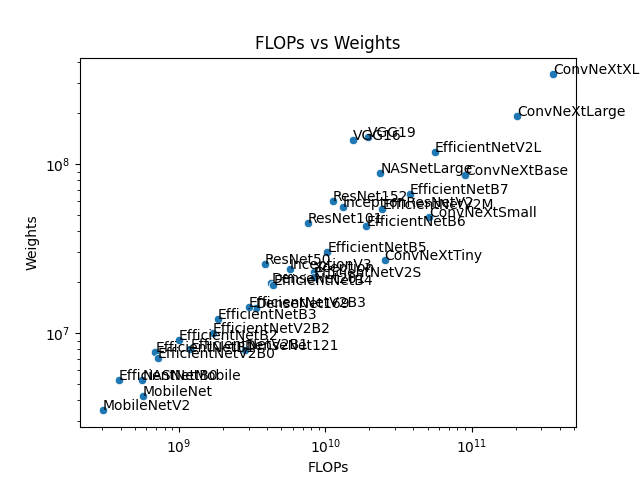
\includegraphics[clip, height=12cm, bb=-60 0 640 480]{data/figure/models_info.png}
		\caption{モデルごとのFLOPsとWeights}
		\label{flops_vs_weights}
	\end{center}
\end{figure}

\subsubsection{AI倫理問題対策の課題}

AIの社会実装において,AIの判断に対して責任を持つことが基本となる.
しかし,AIはブラックボックス的である為,判断根拠を人が解釈することが困難である.

AIを活用する範囲を人が解釈可能な範囲に限定したり,説明可能AI(Explainable AI)技術を活用したりするなどの対策が挙げられる.

% --- T.B.D ---
%市場規模
% 世界市場
%  ✓エッジ型人工知能チップの市場規模は2030年に132億米ドルに達すると予測~最新予測 https://newscast.jp/news/4431496
%  ✓エッジコンピューティング市場規模、2030年に1559億ドル http://www.ex-press.jp/lfwj/lfwj-news/lfwj-biz-market/52519/
%  ✓AIエッジコンピューティング市場、2030年に596億ドル http://ex-press.jp/lfwj/lfwj-news/lfwj-biz-market/45075/
%  ✓エッジ AI プロセッサ市場(Edge AI Processor Market)に関する調査は、2023年の市場のランドスケープを理解するために実施されました。 https://prtimes.jp/main/html/rd/p/000002320.000072515.html
%  ✓エッジ AI ハードウェア市場 - 成長、トレンド、COVID-19 の影響、および予測 (2023 - 2028) https://www.mordorintelligence.com/ja/industry-reports/edge-ai-hardware-market
%  ✓エッジAIソフトウェアの市場規模、2026年に18億3500万米ドル到達予測 https://www.value-press.com/pressrelease/267210
%  ✓エッジAIソフトウェア市場、2027年まで20.3%の成長率を予想 https://aismiley.co.jp/ai_news/edge-ai-software-market-expects-20-3-growth-by-2027/
%  ✓政府機関におけるエッジAIの市場規模、2032年までに30億米ドル到達予測 https://www.mapion.co.jp/news/release/dn0000270836-all/
%  ✓エッジAIコンピューティング市場を予想、2025年度には413億円に拡大 https://news.mynavi.jp/techplus/article/20211214-2227346/
% 国内市場
%  ✓【エッジAIの活用事例】AIカメラからFA機器まで市場規模は拡大の一途 https://standard-dx.com/post_blog/edge-ai
%  ✓本格的な導入が進む国内のAI(人工知能)ビジネス市場を調査 https://www.fuji-keizai.co.jp/press/detail.html?cid=19039
%  ×ミック経済研究所、マーケティング資料「エッジAIコンピューティング市場の実態と将来展望 2021年度版」を発刊 https://www.nikkei.com/article/DGXLRSP623718_U1A211C2000000/
%  ✓国内エッジAI市場は前年比70.8%増、今後の成長ドライバーはAIエンジン─デロイト トーマツ ミック研 https://it.impress.co.jp/articles/-/24005
%  ✓エッジ AI プロセッサ市場(Edge AI Processor Market)に関する調査は、2023年の市場のランドスケープを理解するために実施されました。 https://prtimes.jp/main/html/rd/p/000002320.000072515.html
%  ×データセンター市場及び クラウドサービス市場の動向 https://www.soumu.go.jp/johotsusintokei/whitepaper/ja/r05/pdf/n4800000.pdf
%  ✓AIの拡大と活用動向 https://www.toshiba-dme.co.jp/dme/dig/edge_solution/trend.htm
%  ✓IDC Japan、2023年以降の国内AIシステム市場予測を発表 https://aismiley.co.jp/ai_news/idc-japan-2023/
%  ×富士キメラ総研 AIビジネス国内市場調査 2025年には2兆円規模に拡大 DXに不可欠な要素技術として利用増加 https://www.automation-news.jp/2021/07/57280/
% 技術トレンド
%  ✓2023 年に注目すべきエッジ AI の 5 つのトレンド https://blogs.nvidia.co.jp/2023/01/17/edge-ai-trends-2023/
%  エッジAIカメラの活用から市場動向まで:スマートセキュリティと画像認識技術の最新トレンドを徹底解説 https://www.morphoai.com/post/edge-ai-content
%  エッジAI分野における優位性の獲得 https://www.jp.kearney.com/issue-papers-perspectives/gaining-the-edge-in-edge-ai
%  エッジAI発展に重要な「インメモリコンピューティング」 https://eetimes.itmedia.co.jp/ee/articles/2109/30/news084.html
%  エッジAIとは?5つの活用シーンと10社の開発事例を紹介 https://ainow.ai/2020/02/21/183186/
%  A.T.カーニー、エッジAI市場における勝利の方程式を導く論考「エッジAI分野における優位性の獲得」を公開 https://ledge.ai/articles/kearney-edge-ai
%業界団体
%	TinyML
%
%企業
%  エッジAIカメラの活用から市場動向まで:スマートセキュリティと画像認識技術の最新トレンドを徹底解説 https://www.morphoai.com/post/edge-ai-content
%  TI Edge AI Cloud https://dev.ti.com/edgeai/?utm_source=google&utm_medium=cpc&utm_campaign=epd-null-null-58700008186542725_EdgeAI_Dev_rsa-cpc-pp-google-jp_int&utm_content=EdgeAI_Dev&ds_k=%E3%82%A8%E3%83%83%E3%82%B8+AI&DCM=yes&gclid=Cj0KCQjwuNemBhCBARIsADp74QRb9Mx3n5koyT99HvoPdK97xdrHLeFVCg1WCJ1nEaJagx5JH9giDhsaAlsjEALw_wcB&gclsrc=aw.ds
%  エッジAIコンサルティングサービス https://www.araya.org/service/edgeaiconsulting/?utm_source=google&utm_campaign=edgeai&utm_medium=cpc&gclid=Cj0KCQjwuNemBhCBARIsADp74QR13i96ZIk77RCoSMZfKjfE2cxfO-JxD4RIJ34oPDFb7fzgh9GbIpcaApKhEALw_wcB
%  国内シェアNo.1エッジAIプラットフォーム https://www.idein.jp/ja
%  AI開発に強い開発会社、プロ厳選の21社!【2023年最新版】 https://ai-market.jp/services/ai_development_company/




